\chapter{Resultados} \label{resultados}

  Na\textbf{ Figura \ref{ETHEL}} pode se observar a saída de um dos testes realizados com o ETHEL. Como pode-se constatar foram incluídas as métricas excursão máxima AP (\textit{AMPLITUDE\_AP}) e excursão máxima ML (\textit{AMPLITUDE\_ML}). As métrias são apresentadas no ETHEL em milímetros (mm). Mas para facilitar uma futura comparação dos resultados com o \textit{Posturography Test} Os resultados são apresentadas em centímetros e, podem ser conferidos no \textbf{Apêndice \ref{resultadostestes}}. 


\begin{figure}[ht]
\captionsetup{justification   = raggedright,
              singlelinecheck = false}
\caption{Exemplo da saída dos Testes com ETHEL}\label{ETHEL}
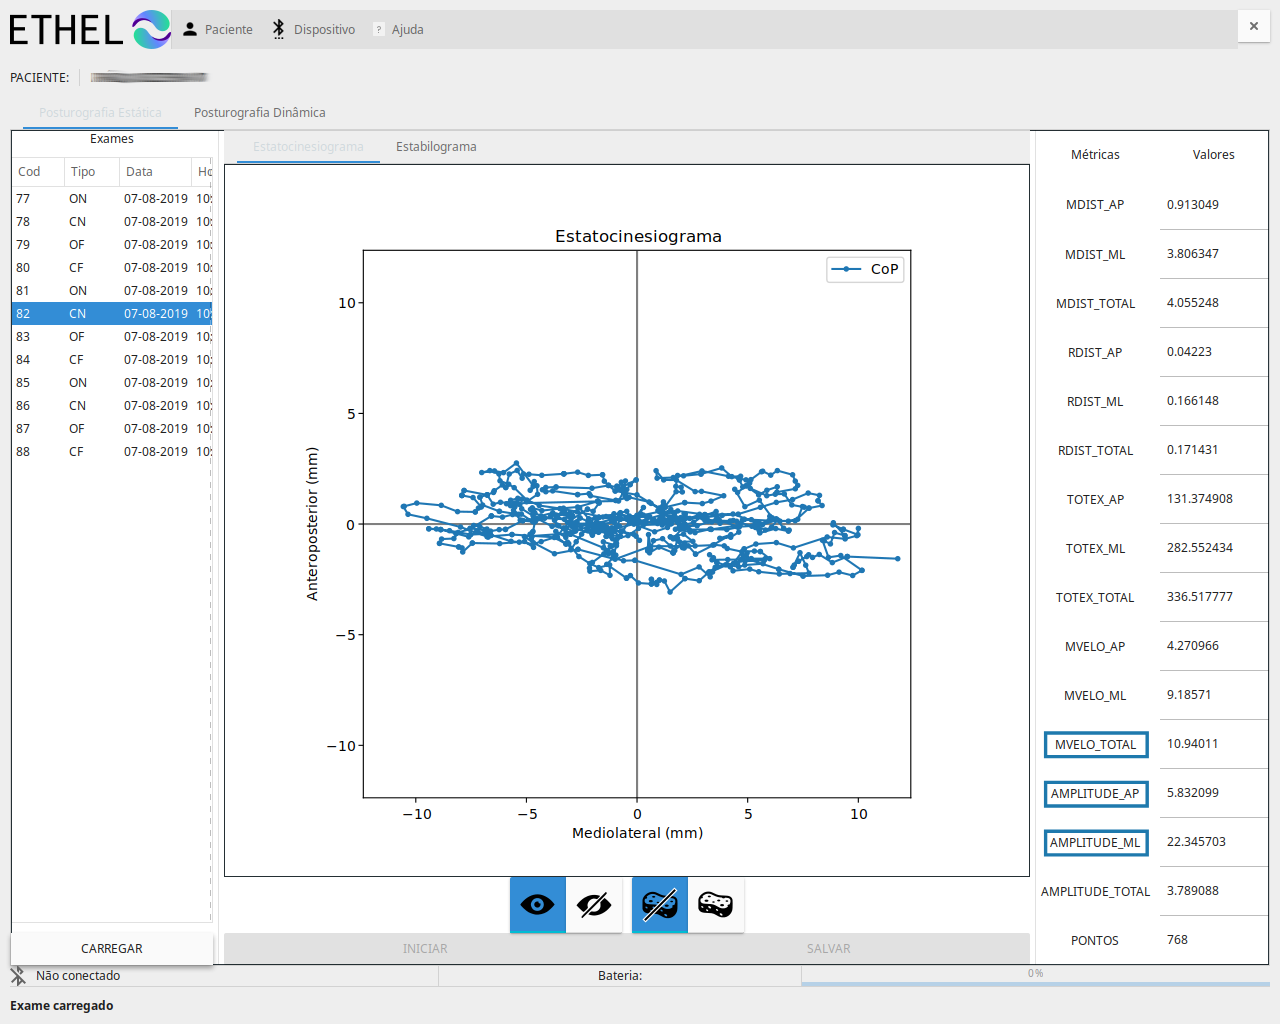
\includegraphics[width=1.0\textwidth]{figs/ETHEL.png}
\end{figure}


Os testes com o LOS não foram apresentados nesta etapa. A interface gráfica foi implementada e já está funcional. Entretanto, ainda que a descrição deste tipo de teste possa ser encontrada na literatura (\citeauthor{tsang2003effects}, \citeyear{tsang2003effects}), as especificações do cálculo das métricas não fica clara no caso do Posturography Test. Assim o processo de implementação deste módulo ainda encontra-se em andamento. Na \textbf{Figura \ref{LOS}} se observa a interface gráfica desenvolvida para o LOS. Os usuários conseguem interagir e movimentar o cursor na tela, deslocando o corpo na direção do alvo proposto.


\begin{figure}[ht]
\captionsetup{justification   = raggedright,
              singlelinecheck = false}
\caption{Interface Gráfica do Módulo dos LOS} \label{LOS}
\begin{center}
	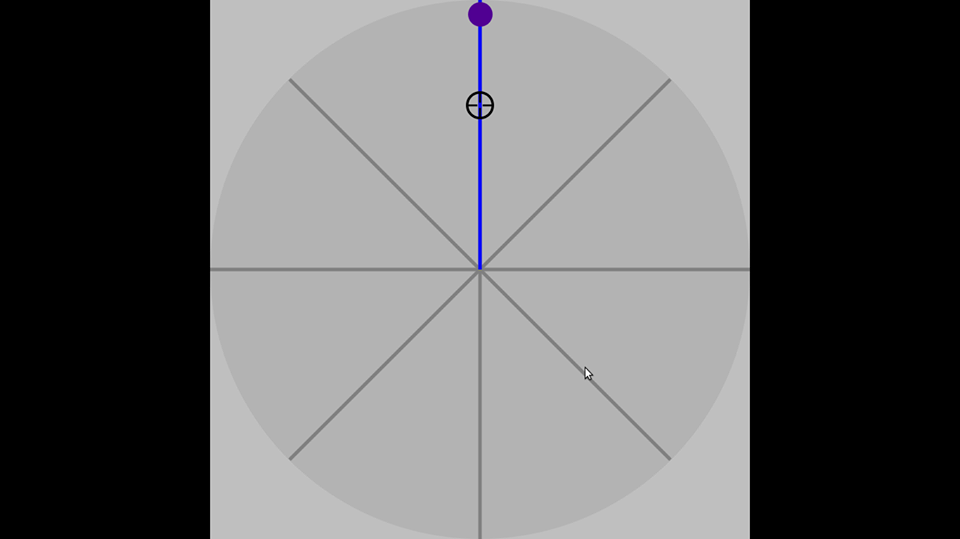
\includegraphics[height=6cm]{figs/LOS1.png} \quad
	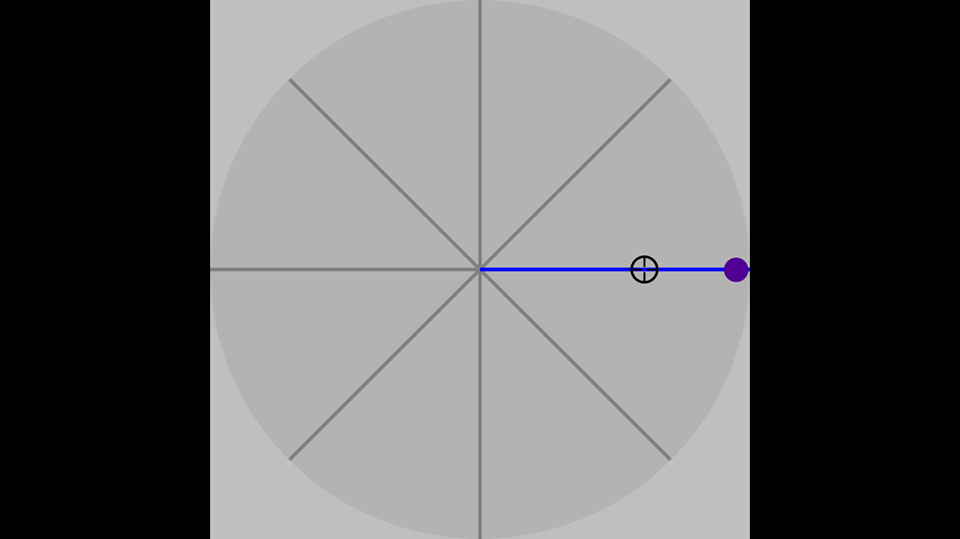
\includegraphics[height=6cm]{figs/LOS2.png}
\end{center}
\end{figure}

De forma geral os testes realizados com cada voluntario, utilizando o ETHEL, demoraram entre 10 e 15 minutos. Neste tempo não foi incluído a realização da avaliação inicial descrita no \textbf{Anexo \ref{anexoCEP}} e, realizada por uma Fisioterapeuta. Esta métrica é importante de ser salientada porque, em testes anteriormente feitos com o \textit{Posturography Test}, a equipe relatou demora para 
finalização do conjunto de testes.

Além da média e do desvio padrão foi  incluído nos resultados (\textbf{Apêndice \ref{resultadostestes}}) o desvio da primeira repetição de cada condição em relação à média das três repetições, na forma de erro relativo. Esta métrica pode ajudar a definir se é necessário ou não a realização de três repetições feitas para cada condição e otimizar o processe de coleta de dados. 

Em posse dos resultados dos testes. A distribuição de frequência do erro relativo é apresentada para cada uma das métricas estimas. Na distribuição de frequência do erro relativo da velocidade média (\textbf{Figura \ref{DistVM}}), observa-se maior frequência entre o terceiro (4,10 - 6,14\%) e quarto (6,14 - 8,20\%) intervalo. Na Excursão Máxima AP (\textbf{Figura \ref{DistAP}}) o primeiro (0 - 4,64\%) e o quarto (13,91 - 18,55\%) intervalo apresentam maior frequência. Na Excursão Máxima ML (\textbf{Figura \ref{DistML}}) o terceiro (9,74 - 14,61\%) intervalo apresentou a maior frequência.



\begin{figure}[ht]
\captionsetup{justification   = raggedright,
              singlelinecheck = false}
\caption{Distribuição de Frequência do Erro Relativo. Velocidade Média.}\label{DistVM}
\includesvg[width=1.0\textwidth]{figs/VM.svg}
\end{figure}

\begin{figure}[ht]
\captionsetup{justification   = raggedright,
              singlelinecheck = false}
\caption{Distribuição de Frequência do Erro Relativo. Excursão Máxima AP.}\label{DistAP}
\includesvg[width=1.0\textwidth]{figs/AP.svg}
\end{figure}

\begin{figure}[ht]
\captionsetup{justification   = raggedright,
              singlelinecheck = false}
\caption{Distribuição de Frequência do Erro Relativo. Excursão Máxima ML.}\label{DistML}
\includesvg[width=1.0\textwidth]{figs/ML.svg}
\end{figure}



A métrica que apresentou o menor desvio padrão e menor erro relativo entre a primeira repetição e a média das repetições, foi a velocidade média. E a que apresentou maior desvio padrão e maior erro relativo, foi a excursão máxima ML (\textbf{Tabela \ref{tabelaMinMeanMax}}). Além disso, quando estimado o melhor e o pior caso, levando em conta métrica e condição sensorial. Temos que o melhor caso, ou seja, o caso que apresentou menor desvio padrão e menor erro relativo. Foi quando calculada a métrica velocidade média na condição sensorial olhos fechados sem espuma. Em  contrapartida, o pior caso foi quando estava estimando a métrica excursão máxima na condição sensorial olhos fechados sobre a espuma (\textbf{Figura \ref{piorMelhor}}).

\newline


% Please add the following required packages to your document preamble:
% \usepackage{booktabs}
\begin{table}[]
 \captionsetup{justification   = raggedright,
              singlelinecheck = false}
 \caption{Desvio Padrão e Erro Relativo. Mínimo, Médio e Máximo.} \label{tabelaMinMeanMax}
\begin{tabular}{@{}lccc@{}}
\toprule
                     & \textbf{Velocidade Média} & \textbf{Excursão Máxima AP} & \textbf{Excursão Máxima ML} \\ \midrule
Desvio Padrão Mínimo & 0,02                      & 0,04                        & 0,19                        \\
Desvio Padrão Médio  & 0,16                      & 0,35                        & 0,56                        \\
Desvio Padrão Máximo & 0,54                      & 1,41                        & 1,80                        \\ \midrule
Erro Mínimo          & 0,64\%                    & 0,83\%                      & 0,95\%                      \\
Erro Médio           & 7,81\%                    & 14,28\%                     & 15,22\%                     \\
Erro Máximo          & 21,15\%                   & 47,21\%                     & 49,68\%                \\  \midrule  
\end{tabular}
\end{table}

\begin{figure}[ht]
\captionsetup{justification   = raggedright,
              singlelinecheck = false}
\caption{Melhor e Pior caso dos testes. Levando em conta métrica estimada e condição sensorial.}\label{piorMelhor}
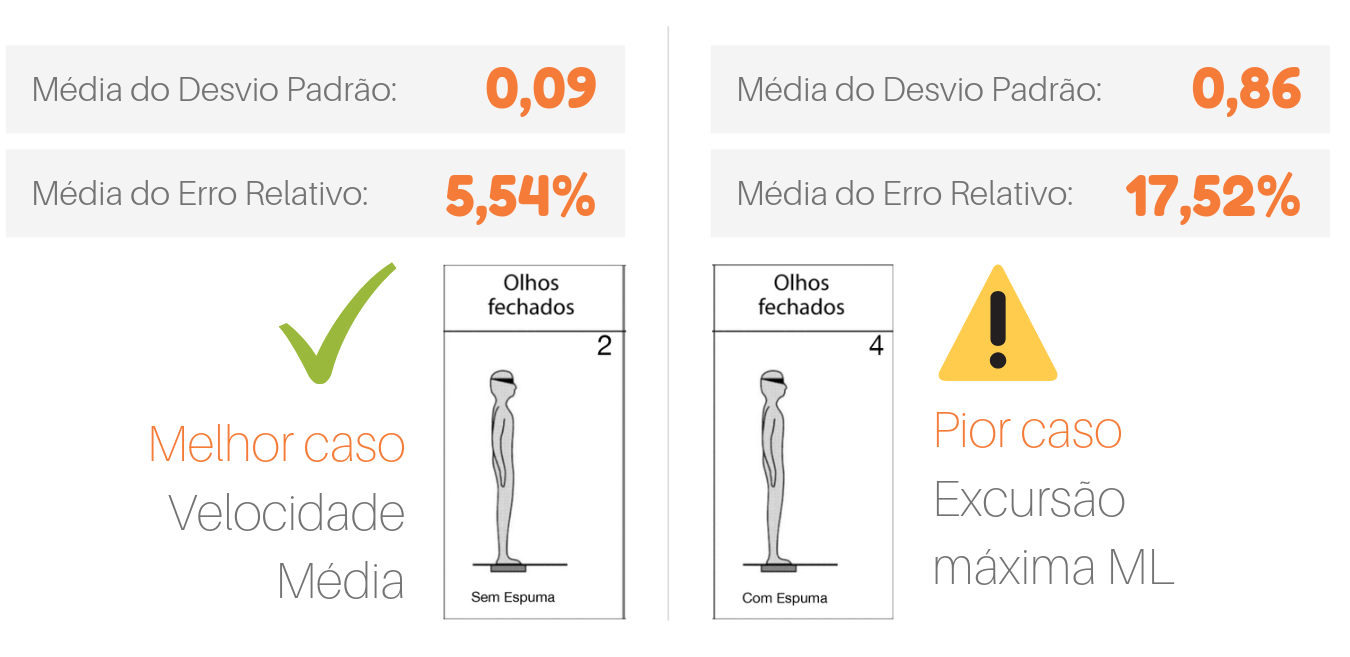
\includegraphics[width=1.0\textwidth]{result.png}
\end{figure}

Os resultados apresentados mostram as inclusões das métricas e da interface gráfica do módulo LOS. Além disso, examina os resultados dos testes realizados. Com objetivo de possibilitar conclusões a respeito da necessidade da realização de três repetições em cada condição sensorial na execução dos teste.


% \begin{longtable}{|c|c|c|c|c|c|}
% \captionsetup{justification   = raggedright,
%               singlelinecheck = false}
% \caption{Resultados testes} \label{tabelaResultados}
% \label{resultadostestes}\\
% \hline
% \textbf{Paciente}   & \textbf{Teste}                             & \textbf{Condição} & \textbf{Média} & \textbf{Desvio} & \textbf{Erro} \\
% & & & & \textbf{Padrão} & \textbf{(\%)} \\ \hline
% \endfirsthead
% %
% \endhead
% \multirow{12}{*}{1} & \multirow{4}{*}{Velocidade Média (cm/seg)} & OASP              & 1,18           & 0,10                   & 9,42               \\ \cline{3-6} 
%                     &                                            & OFSP              & 1,30           & 0,03                   & 0,97               \\ \cline{3-6} 
%                     &                                            & OASE              & 1,76           & 0,09                   & 5,20               \\ \cline{3-6} 
%                     &                                            & OFSE              & 2,60           & 0,23                   & 9,75               \\ \cline{2-6} 
%                     & \multirow{4}{*}{Excursão Máxima AP (cm)}   & OASP              & 0,69           & 0,28                   & 42,28              \\ \cline{3-6} 
%                     &                                            & OFSP              & 0,94           & 0,12                   & 2,87               \\ \cline{3-6} 
%                     &                                            & OASE              & 1,66           & 0,48                   & 8,95               \\ \cline{3-6} 
%                     &                                            & OFSE              & 2,66           & 0,44                   & 10,89              \\ \cline{2-6} 
%                     & \multirow{4}{*}{Excursão Máxima ML (cm)}   & OASP              & 1,70           & 0,21                   & 12,16              \\ \cline{3-6} 
%                     &                                            & OFSP              & 1,57           & 0,71                   & 49,68              \\ \cline{3-6} 
%                     &                                            & OASE              & 3,31           & 0,40                   & 13,05              \\ \cline{3-6} 
%                     &                                            & OFSE              & 4,21           & 0,60                   & 14,01              \\ \hline
% \multirow{12}{*}{2} & \multirow{4}{*}{Velocidade Média (cm/seg)} & OASP              & 1,41           & 0,24                   & 18,67              \\ \cline{3-6} 
%                     &                                            & OFSP              & 1,59           & 0,15                   & 7,29               \\ \cline{3-6} 
%                     &                                            & OASE              & 1,97           & 0,23                   & 11,66              \\ \cline{3-6} 
%                     &                                            & OFSE              & 3,82           & 0,59                   & 3,47               \\ \cline{2-6} 
%                     & \multirow{4}{*}{Excursão Máxima AP (cm)}   & OASP              & 1,22           & 0,32                   & 20,58              \\ \cline{3-6} 
%                     &                                            & OFSP              & 1,54           & 0,25                   & 16,15              \\ \cline{3-6} 
%                     &                                            & OASE              & 1,91           & 0,44                   & 17,61              \\ \cline{3-6} 
%                     &                                            & OFSE              & 2,99           & 0,40                   & 14,64              \\ \cline{2-6} 
%                     & \multirow{4}{*}{Excursão Máxima ML (cm)}   & OASP              & 2,79           & 0,19                   & 7,50               \\ \cline{3-6} 
%                     &                                            & OFSP              & 2,82           & 0,78                   & 30,53              \\ \cline{3-6} 
%                     &                                            & OASE              & 2,77           & 0,43                   & 1,77               \\ \cline{3-6} 
%                     &                                            & OFSE              & 5,32           & 1,33                   & 28,79              \\ \hline
% \multirow{12}{*}{3} & \multirow{4}{*}{Velocidade Média (cm/seg)} & OASP              & 1,28           & 0,05                   & 3,27               \\ \cline{3-6} 
%                     &                                            & OFSP              & 1,35           & 0,08                   & 4,75               \\ \cline{3-6} 
%                     &                                            & OASE              & 1,62           & 0,39                   & 13,39              \\ \cline{3-6} 
%                     &                                            & OFSE              & 1,87           & 0,13                   & 7,61               \\ \cline{2-6} 
%                     & \multirow{4}{*}{Excursão Máxima AP (cm)}   & OASP              & 1,24           & 0,17                   & 11,46              \\ \cline{3-6} 
%                     &                                            & OFSP              & 1,18           & 0,16                   & 2,07               \\ \cline{3-6} 
%                     &                                            & OASE              & 1,66           & 0,25                   & 13,13              \\ \cline{3-6} 
%                     &                                            & OFSE              & 1,42           & 0,04                   & 2,36               \\ \cline{2-6} 
%                     & \multirow{4}{*}{Excursão Máxima ML (cm)}   & OASP              & 2,19           & 0,26                   & 12,96              \\ \cline{3-6} 
%                     &                                            & OFSP              & 2,92           & 0,43                   & 11,64              \\ \cline{3-6} 
%                     &                                            & OASE              & 3,19           & 0,78                   & 2,97               \\ \cline{3-6} 
%                     &                                            & OFSE              & 4,26           & 0,89                   & 21,45              \\ \hline
% \multirow{12}{*}{4} & \multirow{4}{*}{Velocidade Média (cm/seg)} & OASP              & 1,10           & 0,02                   & 2,05               \\ \cline{3-6} 
%                     &                                            & OFSP              & 1,20           & 0,03                   & 1,67               \\ \cline{3-6} 
%                     &                                            & OASE              & 1,42           & 0,16                   & 12,53              \\ \cline{3-6} 
%                     &                                            & OFSE              & 2,18           & 0,37                   & 18,18              \\ \cline{2-6} 
%                     & \multirow{4}{*}{Excursão Máxima AP (cm)}   & OASP              & 0,79           & 0,12                   & 9,99               \\ \cline{3-6} 
%                     &                                            & OFSP              & 0,74           & 0,09                   & 13,59              \\ \cline{3-6} 
%                     &                                            & OASE              & 1,63           & 0,40                   & 22,72              \\ \cline{3-6} 
%                     &                                            & OFSE              & 2,10           & 0,93                   & 3,47               \\ \cline{2-6} 
%                     & \multirow{4}{*}{Excursão Máxima ML (cm)}   & OASP              & 2,20           & 0,35                   & 12,48              \\ \cline{3-6} 
%                     &                                            & OFSP              & 2,27           & 0,43                   & 10,81              \\ \cline{3-6} 
%                     &                                            & OASE              & 3,14           & 0,24                   & 3,37               \\ \cline{3-6} 
%                     &                                            & OFSE              & 4,82           & 1,80                   & 28,24              \\ \hline
% \multirow{12}{*}{5} & \multirow{4}{*}{Velocidade Média (cm/seg)} & OASP              & 1,07           & 0,09                   & 6,53               \\ \cline{3-6} 
%                     &                                            & OFSP              & 1,33           & 0,23                   & 15,26              \\ \cline{3-6} 
%                     &                                            & OASE              & 1,63           & 0,10                   & 4,62               \\ \cline{3-6} 
%                     &                                            & OFSE              & 2,48           & 0,25                   & 10,86              \\ \cline{2-6} 
%                     & \multirow{4}{*}{Excursão Máxima AP (cm)}   & OASP              & 1,55           & 0,27                   & 0,83               \\ \cline{3-6} 
%                     &                                            & OFSP              & 1,58           & 0,33                   & 15,93              \\ \cline{3-6} 
%                     &                                            & OASE              & 2,21           & 0,40                   & 3,54               \\ \cline{3-6} 
%                     &                                            & OFSE              & 2,15           & 0,61                   & 2,65               \\ \cline{2-6} 
%                     & \multirow{4}{*}{Excursão Máxima ML (cm)}   & OASP              & 2,41           & 0,19                   & 6,84               \\ \cline{3-6} 
%                     &                                            & OFSP              & 3,11           & 0,30                   & 9,67               \\ \cline{3-6} 
%                     &                                            & OASE              & 3,04           & 0,62                   & 14,67              \\ \cline{3-6} 
%                     &                                            & OFSE              & 3,85           & 0,66                   & 13,70              \\ \hline
% \multirow{12}{*}{6} & \multirow{4}{*}{Velocidade Média (cm/seg)} & OASP              & 1,66           & 0,08                   & 5,61               \\ \cline{3-6} 
%                     &                                            & OFSP              & 1,88           & 0,11                   & 6,41               \\ \cline{3-6} 
%                     &                                            & OASE              & 1,81           & 0,13                   & 0,95               \\ \cline{3-6} 
%                     &                                            & OFSE              & 2,68           & 0,33                   & 0,64               \\ \cline{2-6} 
%                     & \multirow{4}{*}{Excursão Máxima AP (cm)}   & OASP              & 1,38           & 0,11                   & 8,85               \\ \cline{3-6} 
%                     &                                            & OFSP              & 1,57           & 0,18                   & 12,92              \\ \cline{3-6} 
%                     &                                            & OASE              & 1,62           & 0,27                   & 7,59               \\ \cline{3-6} 
%                     &                                            & OFSE              & 1,70           & 0,27                   & 14,75              \\ \cline{2-6} 
%                     & \multirow{4}{*}{Excursão Máxima ML (cm)}   & OASP              & 3,25           & 0,60                   & 14,01              \\ \cline{3-6} 
%                     &                                            & OFSP              & 3,14           & 0,66                   & 13,07              \\ \cline{3-6} 
%                     &                                            & OASE              & 2,42           & 0,25                   & 11,13              \\ \cline{3-6} 
%                     &                                            & OFSE              & 4,63           & 0,54                   & 6,14               \\ \hline
% \multirow{12}{*}{7} & \multirow{4}{*}{Velocidade Média (cm/seg)} & OASP              & 0,87           & 0,09                   & 7,97               \\ \cline{3-6} 
%                     &                                            & OFSP              & 1,04           & 0,06                   & 6,33               \\ \cline{3-6} 
%                     &                                            & OASE              & 1,09           & 0,10                   & 4,24               \\ \cline{3-6} 
%                     &                                            & OFSE              & 1,82           & 0,14                   & 5,31               \\ \cline{2-6} 
%                     & \multirow{4}{*}{Excursão Máxima AP (cm)}   & OASP              & 0,84           & 0,33                   & 17,40              \\ \cline{3-6} 
%                     &                                            & OFSP              & 0,52           & 0,13                   & 16,36              \\ \cline{3-6} 
%                     &                                            & OASE              & 1,00           & 0,25                   & 14,55              \\ \cline{3-6} 
%                     &                                            & OFSE              & 1,48           & 0,13                   & 4,64               \\ \cline{2-6} 
%                     & \multirow{4}{*}{Excursão Máxima ML (cm)}   & OASP              & 1,85           & 0,19                   & 8,18               \\ \cline{3-6} 
%                     &                                            & OFSP              & 2,07           & 0,23                   & 12,82              \\ \cline{3-6} 
%                     &                                            & OASE              & 1,90           & 0,30                   & 0,95               \\ \cline{3-6} 
%                     &                                            & OFSE              & 3,26           & 0,29                   & 6,82               \\ \hline
% \multirow{12}{*}{8} & \multirow{4}{*}{Velocidade Média (cm/seg)} & OASP              & 1,21           & 0,12                   & 6,42               \\ \cline{3-6} 
%                     &                                            & OFSP              & 1,35           & 0,09                   & 2,63               \\ \cline{3-6} 
%                     &                                            & OASE              & 1,56           & 0,07                   & 4,86               \\ \cline{3-6} 
%                     &                                            & OFSE              & 2,53           & 0,34                   & 15,60              \\ \cline{2-6} 
%                     & \multirow{4}{*}{Excursão Máxima AP (cm)}   & OASP              & 1,60           & 0,45                   & 1,27               \\ \cline{3-6} 
%                     &                                            & OFSP              & 1,38           & 0,43                   & 19,27              \\ \cline{3-6} 
%                     &                                            & OASE              & 2,24           & 0,75                   & 8,39               \\ \cline{3-6} 
%                     &                                            & OFSE              & 3,08           & 1,41                   & 47,21              \\ \cline{2-6} 
%                     & \multirow{4}{*}{Excursão Máxima ML (cm)}   & OASP              & 2,28           & 0,64                   & 31,49              \\ \cline{3-6} 
%                     &                                            & OFSP              & 2,64           & 0,73                   & 20,94              \\ \cline{3-6} 
%                     &                                            & OASE              & 2,43           & 0,47                   & 7,39               \\ \cline{3-6} 
%                     &                                            & OFSE              & 3,96           & 0,86                   & 24,55              \\ \hline
% \multirow{12}{*}{9} & \multirow{4}{*}{Velocidade Média (cm/seg)} & OASP              & 0,96           & 0,08                   & 7,51               \\ \cline{3-6} 
%                     &                                            & OFSP              & 1,19           & 0,05                   & 4,58               \\ \cline{3-6} 
%                     &                                            & OASE              & 1,36           & 0,26                   & 21,15              \\ \cline{3-6} 
%                     &                                            & OFSE              & 1,97           & 0,24                   & 14,08              \\ \cline{2-6} 
%                     & \multirow{4}{*}{Excursão Máxima AP (cm)}   & OASP              & 0,87           & 0,23                   & 30,47              \\ \cline{3-6} 
%                     &                                            & OFSP              & 1,00           & 0,40                   & 30,35              \\ \cline{3-6} 
%                     &                                            & OASE              & 1,23           & 0,24                   & 22,67              \\ \cline{3-6} 
%                     &                                            & OFSE              & 1,88           & 0,36                   & 21,70              \\ \cline{2-6} 
%                     & \multirow{4}{*}{Excursão Máxima ML (cm)}   & OASP              & 1,46           & 0,37                   & 21,54              \\ \cline{3-6} 
%                     &                                            & OFSP              & 2,12           & 0,77                   & 6,66               \\ \cline{3-6} 
%                     &                                            & OASE              & 2,07           & 0,76                   & 41,99              \\ \cline{3-6} 
%                     &                                            & OFSE              & 4,56           & 0,80                   & 13,96              \\ \hline
% \end{longtable}

